\chapter{Resultados}
\label{cap:Resultados_init}
\section{Correção de camera}
\label{sec:Resultados_correcao_camera}

Nesta seção apresenta-se os resultados dos trabalhos realizado a cerca da correção de efeitos de camera.
Apesar do trabalho utilizar apenas simulações, esta simulação também apresenta distorções.
Como observa-se na figura \ref{fig:distortion} as estrelas mais distantes do centro do frame da camera estão distante do plano da imagem,
o que gera o e efeito de distorção radial.

\begin{figure}[H]
    \centering
    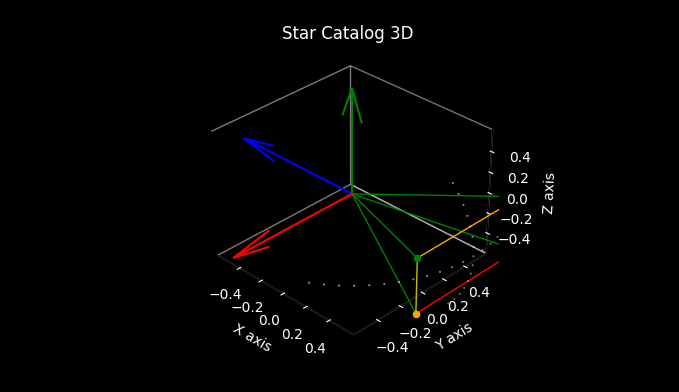
\includegraphics[width=1\textwidth]{images/distortion.png}
    \caption{Visualização do erro espacial de distorção radial. Fonte: Autoria própria}
    \label{fig:distortion}
\end{figure}

Para realizara corre da correção no simulador, foi utilizado uma base da dados de calibração da camera,
que consiste em estrelas com relação angular conhecida,
neste caso estrelas com 5 graus de separação angular entre si,
o que resulta no frame Visto na figura \ref{fig:Camera_conhecido}.

\begin{figure}[H]
    \centering
    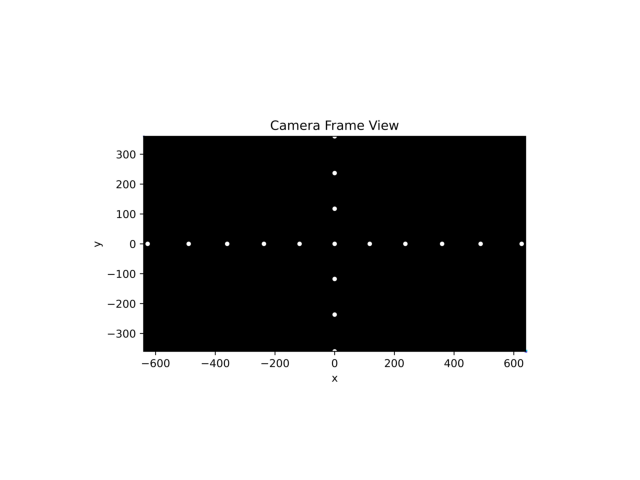
\includegraphics[width=1\textwidth]{images/Camera_conhecido.png}
    \caption{Visualização do frame da camera com estrelas conhecidas. Fonte: Autoria própria}
    \label{fig:Camera_conhecido}
\end{figure}

Os dados da figura \ref{fig:Camera_conhecido} são colocados no algoritmo de detecção de centroides para encontrar a distancia medida das estrelas até o centro da imagem,
além disto é calculado a média das distancias medidas de estrelas com mesma distancia até o centro da imagem, para reduzir o erro de medição.
Com isto podemos comparar ao valor esperado caso a camera não apresentasse distorção radial,
neste trabalho considera-se que a medida real é o valor medido da estrela da estrela mais proxima ao centro da imagem.
Com isto pode-se comparar o valor medido com o valor esperado, que é visto na figura \ref{fig:comparacoes_de_erro}.

\begin{figure}[H]
    \centering
    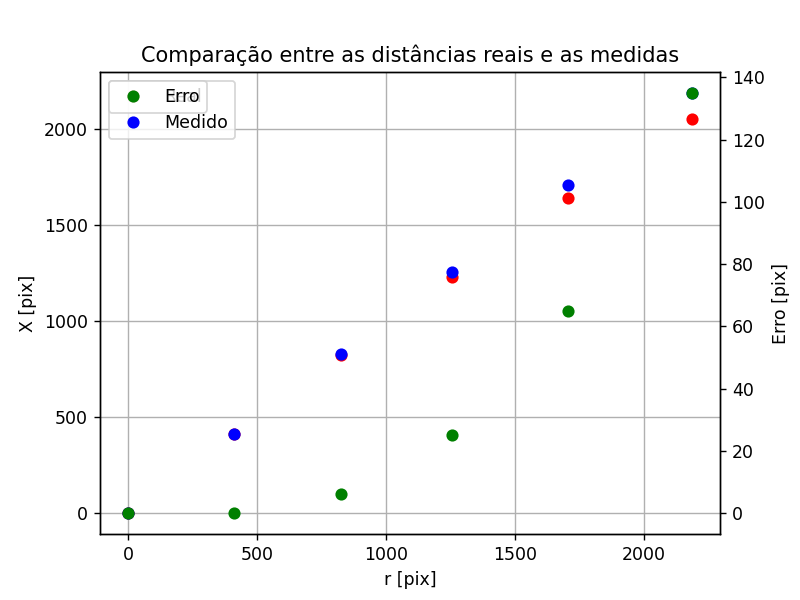
\includegraphics[width=0.5\textwidth]{images/comparacoes_de_erro.png}
    \caption{Visualização do erro espacial de distorção radial. Fonte: Autoria própria}
    \label{fig:comparacoes_de_erro}
\end{figure}

Como o esperado o erro segue uma reta polinomial, como explicado na seção \ref{subsubsec:distorcao_radial}, com os representados mostrados na figura \ref{fig:image_corretion}.
Com o polinômio de ajuste resultante possuindo as constantes \ref{eq:result_image1},\ref{eq:result_image2},\ref{eq:result_image3}, 

\begin{equation}
    K1 = -9.6415774825692e-09\newline
    \label{eq:result_image1}
\end{equation}

\begin{equation}
    K2 = -2.0788174598076455e-15,
    \label{eq:result_image2}
\end{equation}

\begin{equation}
    K3 = 2.910928744425903e-22.
    \label{eq:result_image3}
\end{equation}

Aplicação das correções resulta na figura \ref{fig:image_corretion}, 
que mostra que a correção foi bem sucedida, pois o erro que estava em até 120 pixel agora está em até 1 pixel.

\begin{figure}[H]
    \centering
    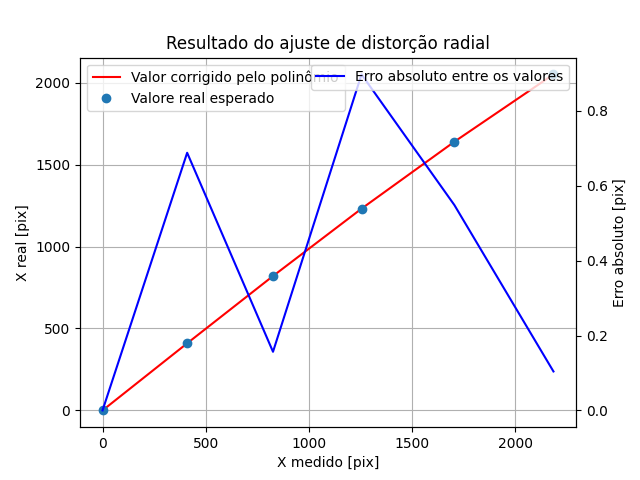
\includegraphics[width=0.5\textwidth]{images/image_corretion.png}
    \caption{Resultado da correção radial. Fonte: Autoria própria}
    \label{fig:image_corretion}
\end{figure}

\section{Aplicação do algoritmo k vector para pesquisa no banco de dados}

A plicação do algoritmo k vector para criação de um banco de dados mais eficiente, 
foi realizada com a lista de ângulos entre estrelas, 
na Figura \ref{fig:k_vector_angulos} é mostrado o resultado para a aplicação utilizando um polinômio de grau 2.

Originalmente o vetor possui mais de 400 mil elementos, com a utilização do algoritmo k vector, 
o vetor de pesquisa é reduzido a 2 * o erro máximo, que de neste caso se torna um vetor menor de 4 mil elementos.
O que é uma redução para menos de 1\% do tamanho original.

\begin{figure}[H]
    \centering
    \includegraphics[width=1\textwidth]{images/k_vector_angulos.png}
    \caption{Resultado da aplicação do algoritmo k vector para o banco de dados de ângulos. Fonte: Autoria própria}
    \label{fig:k_vector_angulos}
\end{figure}

\section{Localização de estrelas}

Os resultados obtidos em simulação, 
indicam que o sistema tem potencial para ser utilizado em cubesats reais como foi proposto inicialmente,
pois o algoritmo se mostra rápido e robusto, conseguindo indentificar as estrelas presentes no FOV(\textit{Field of View}) na maioria dos testes. 
Na tabela ~\ref{tab:tempo_de_execucao_img} é possível observar o tempo em que o algoritmo leva para executar, 
a análise da imagem em si, o que envolve a aplicação do filtro do borda de Canny, a utilização da transformada de Hough e a detecção de círculos,
e o calculo das relações angulares e geométricas entre as estrelas.

A tabela ~\ref{tab:tempo_de_execucao_db} mostra o tempo de execução da busca no banco de dados,
resultando que esta aplicação realiza a busca para o caso em que o cubesat não possui nenhuma informação anterior sobre a sua posição.

Cabe ressaltar que a terminação final da atitude do cubesat ainda exige a implementação de um algoritmo que relacione a estrela visualizada com a sua posição no espaço.

\begin{table}[ht]
    \centering

    \begin{tabular}{|c|c|c|c|c|}
        \hline
        \textbf{Roll (dec º)} & \textbf{Acensão (dec º)} & \textbf{Declinação (dec º)} & \textbf{Tempo analise de imagem (s)} \\ \hline
        0                     & 0                        & 0                           & 1.760                                \\ \hline
        191                   & 170                      & 79                          & 0.770                                \\ \hline
        11                    & 31                       & 44                          & 0.903                                \\ \hline
        92                    & 105                      & 50                          & --                                   \\ \hline
        264                   & 159                      & -63                         & 6.393                                \\ \hline
    \end{tabular}
    \caption{Tempo de execução do algoritmo de análise de imagem, Fonte: Autoria própria}
    \label{tab:tempo_de_execucao_img}
\end{table}

\begin{table}[ht]
    \centering

    \begin{tabular}{|c|c|c|c|c|}
        \hline
        \textbf{Roll (dec º)} & \textbf{Acensão (dec º)} & \textbf{declinação (dec º)} & \textbf{Tempo de busca (s)} \\ \hline
        0                     & 0                        & 0                           & 0.362                       \\ \hline
        191                   & 170                      & 79                          & 3.457                       \\ \hline
        11                    & 31                       & 44                          & 1.132                       \\ \hline
        92                    & 105                      & 50                          & --                          \\ \hline
        264                   & 159                      & -63                         & 2.116                       \\ \hline
    \end{tabular}
    \caption{Tempo de execução da pesquisa no banco de dados, Fonte: Autoria própria}
    \label{tab:tempo_de_execucao_db}
\end{table}

A linha em que o tempo de análise de imagem é "--" indica que o sistema não consegui determinar quais estrelas estavam sendo analisada no FOV. 
Junto a análise de tempo de execução, é realizada a analise de acurácia do sistema,
verificando se o sistema detectou corretamente as estrelas presentes no FOV.

A analise é realizada da seguinte forma, primeiramente gera-se um frame aleatório, através do \textit{software} de simulação,
após isto, o frame é analisado pelo \textit{software} do cubesat que gera uma lista de IDs das possíveis estrelas encontradas no FOV.
Com está informação é então criado um novo \textit{set} de estrelas contendo apenas as estrelas localizadas pelo \textit{software} do cubesat.

Este novo \textit{set} refinado de estrelas é carregado no \textit{software} de simulação e é então gerado um novo frame, quando então é comparado se o novo frame é compatível com o frame gerado anteriormente. 
A Tabela ~\ref{tab:acuracia} mostra os resultados obtidos, 
pode-se ter 3 resultados distintos:

\begin{itemize}
    \item \textbf{Correto}: o sistema detectou corretamente as estrelas presentes no FOV;
    \item \textbf{Incorreto}: o sistema detectou incorretamente as estrelas presentes no FOV;
    \item \textbf{Inconclusivo}: o sistema não detectou todas as estrelas presentes no FOV.
\end{itemize}

\begin{table}[ht]
    \centering

    \begin{tabular}{|c|c|c|c|c|}
        \hline
        \textbf{Roll (dec º)} & \textbf{Acensão (dec º)} & \textbf{declinação (dec º)} & \textbf{Resultado} \\ \hline
        0                     & 0                        & 0                           & Correto            \\ \hline
        191                   & 170                      & 79                          & Correto            \\ \hline
        11                    & 31                       & 44                          & Incorreto          \\ \hline
        92                    & 105                      & 50                          & Inconclusivo       \\ \hline
        264                   & 159                      & -63                         & Correto            \\ \hline
    \end{tabular}
    \caption{Acurácia do sistema, Fonte: Autoria própria}
    \label{tab:acuracia}
\end{table}

Para reforçar os resultados obtidos as figuras ~\ref{fig:errou}, ~\ref{fig:errou_2D}, ~\ref{fig:errou_3D}, ~\ref{fig:acertou},~\ref{fig:acertou_2D} e ~\ref{fig:acertou_3D} mostram os resultados obtidos para os casos em que o sistema detectou incorretamente e corretamente as estrelas presentes no FOV.

Para se considerar que o sistema detectou corretamente ou não as estrelas presentes no FOV, 
é realizado a construção de um \textit{sub-set} apenas com as estrelas detectadas, 
se o novo frame gerado a partir do \textit{sub-set} possuir as estrelas selecionadas no mesmo ponto do frame anterior, 
então o teste é considerado como correto, caso contrário é considerado como incorreto.
Teste inconclusivo é quando o sistema não retorna nenhuma estrela em especifico como solução. 

\begin{figure}[H]
    \centering
    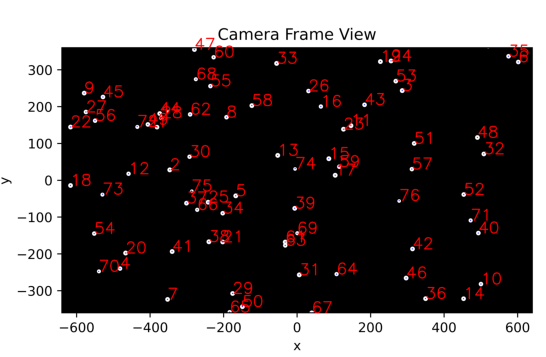
\includegraphics[width=1\textwidth]{images/errou.png}
    \caption{Resultado obtido para o caso em que o sistema detectou incorretamente as estrelas presentes no FOV, Fonte: Autoria própria}
    \label{fig:errou}
\end{figure}

\begin{figure}[H]
    \centering
    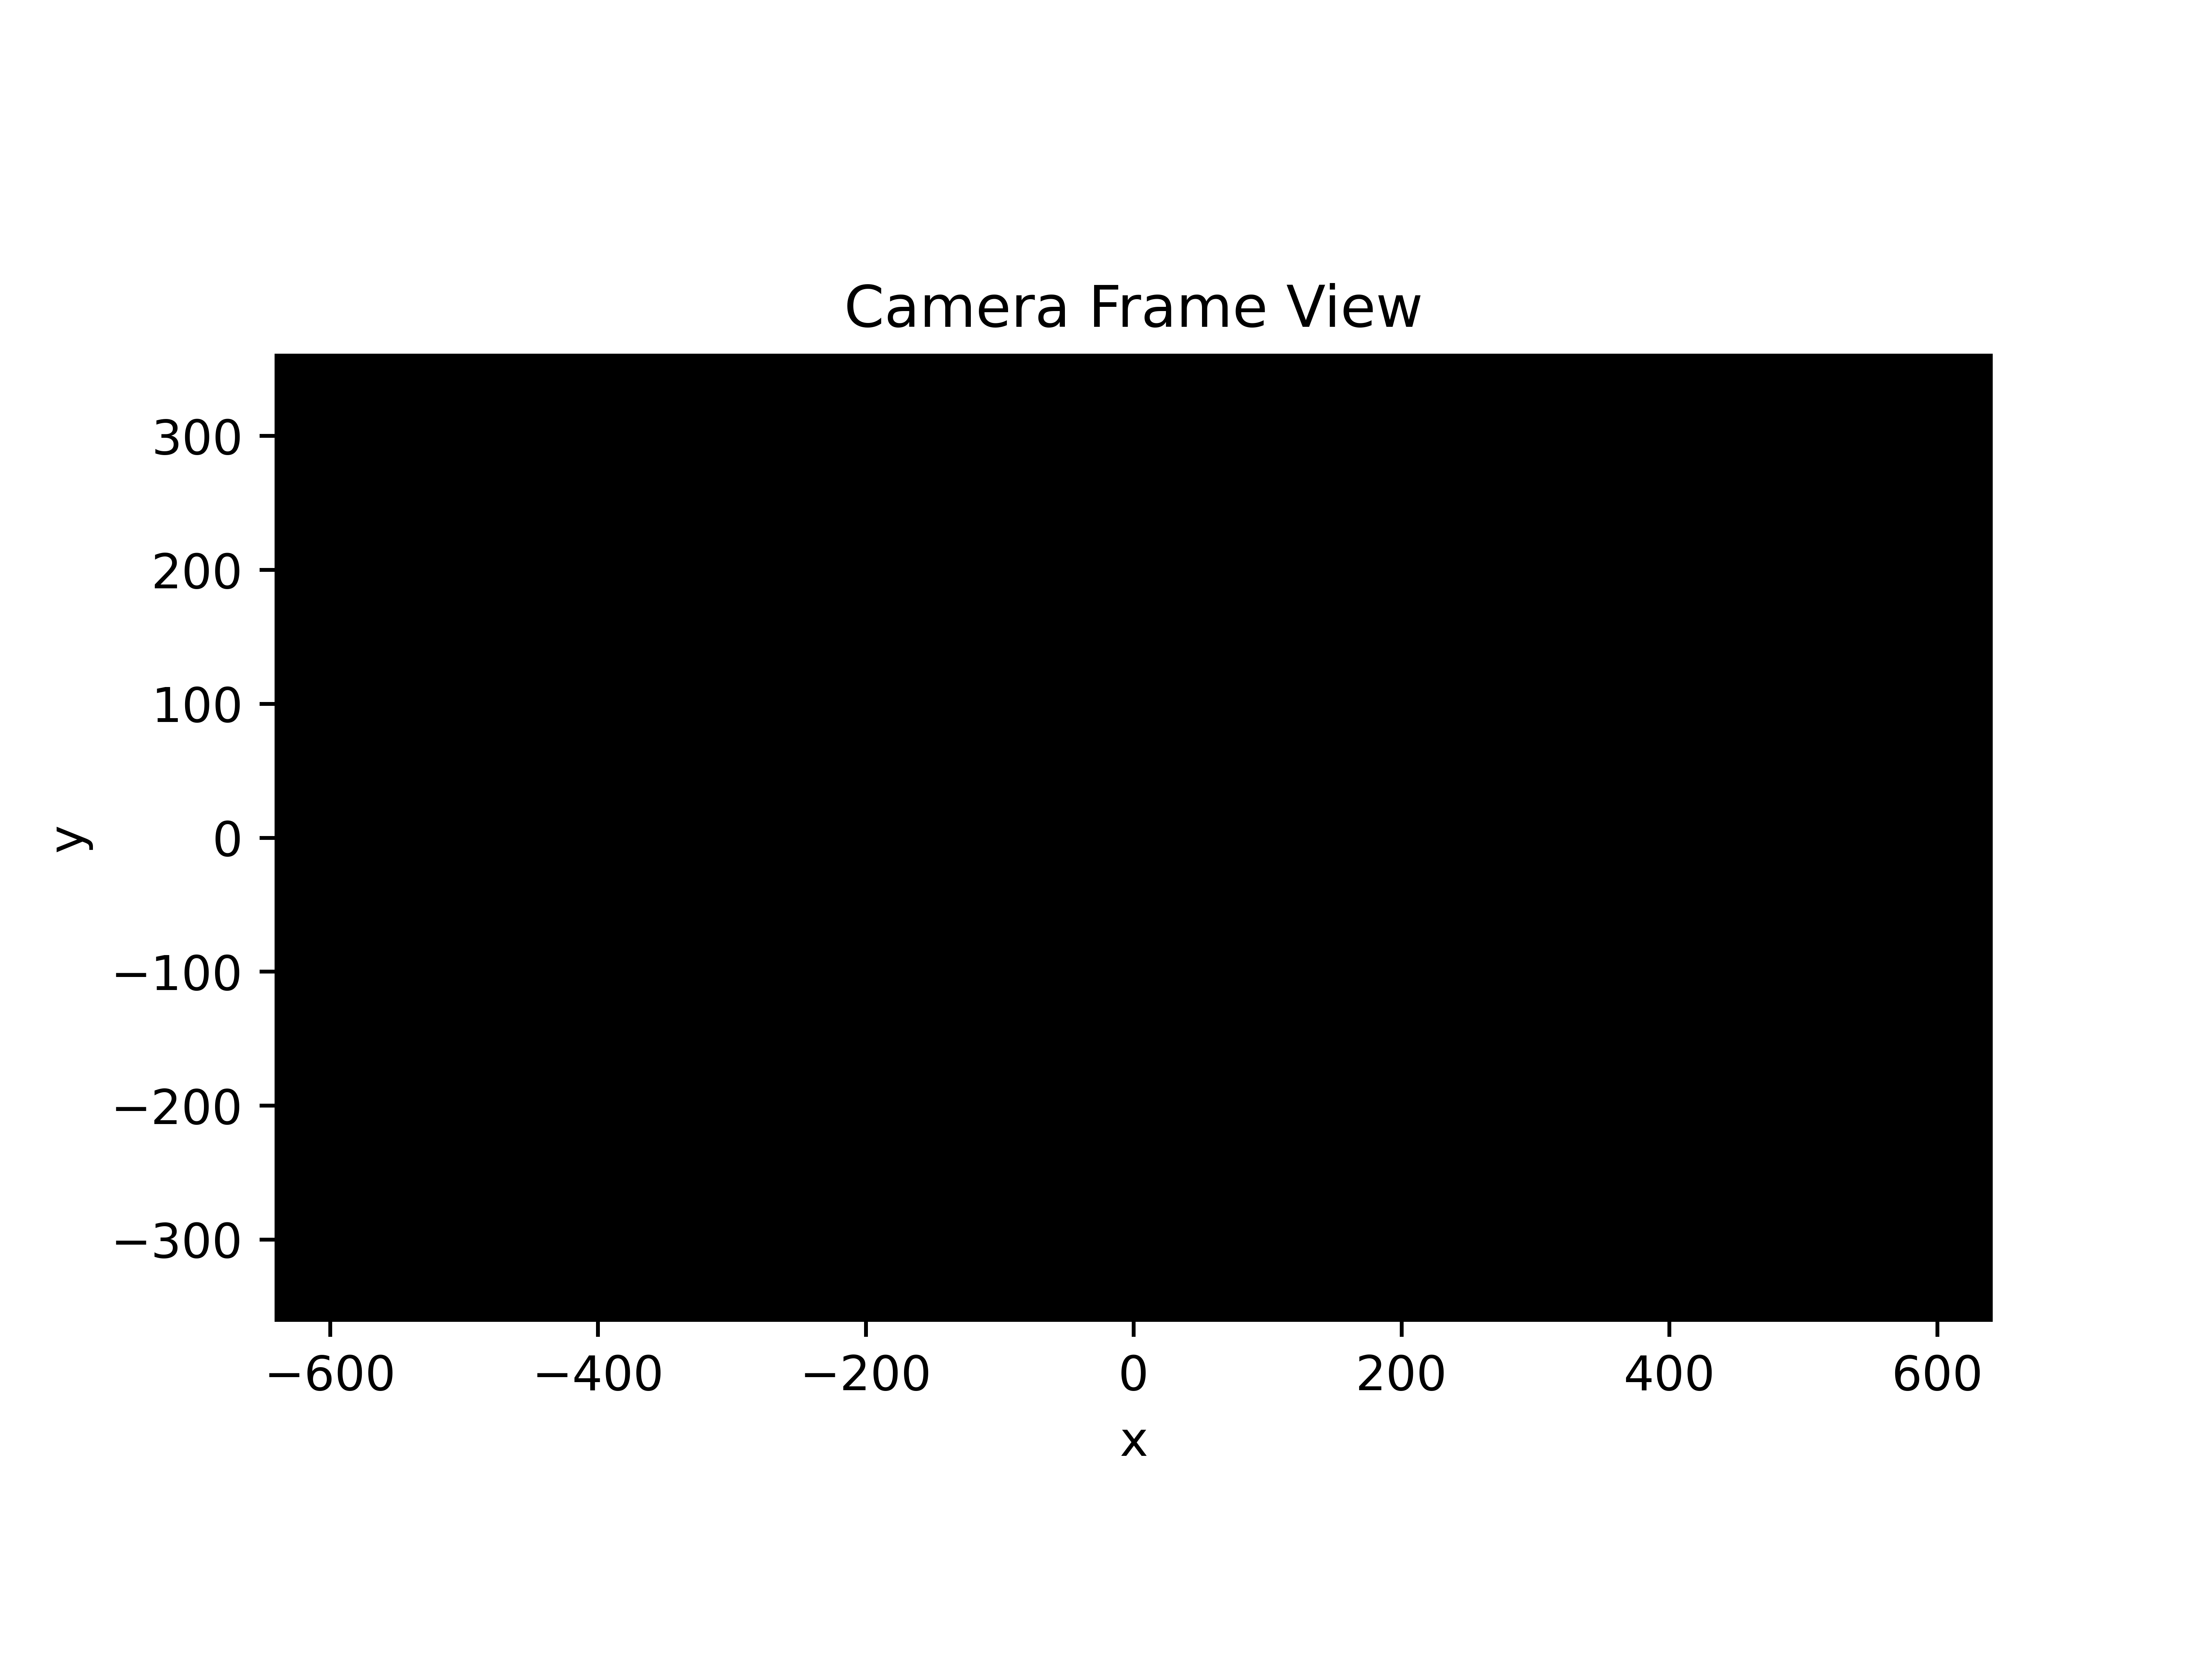
\includegraphics[width=1\textwidth]{images/errou_2D.png}
    \caption{Resultado obtido para o caso em que o sistema detectou incorretamente as estrelas presentes no FOV, Fonte: Autoria própria}
    \label{fig:errou_2D}
\end{figure}

\begin{figure}[H]
    \centering
    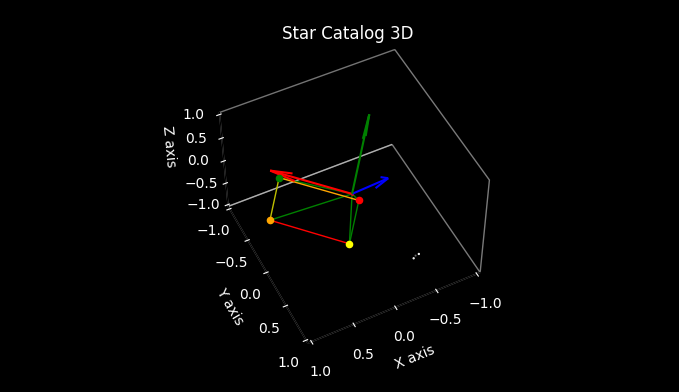
\includegraphics[width=1\textwidth]{images/errou_3D.png}
    \caption{Resultado obtido para o caso em que o sistema detectou incorretamente as estrelas presentes no FOV, Fonte: Autoria própria}
    \label{fig:errou_3D}
\end{figure}

\begin{figure}[H]
    \centering
    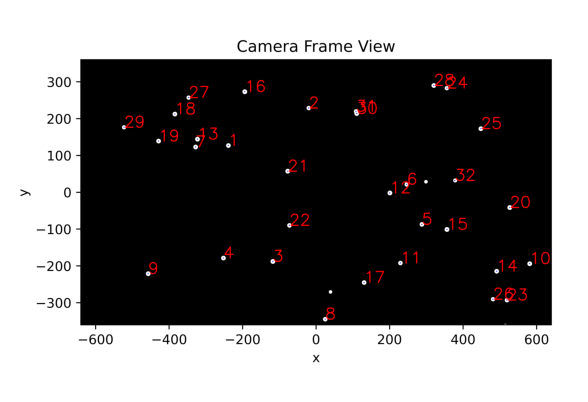
\includegraphics[width=1\textwidth]{images/acertou.png}
    \caption{Resultado obtido para o caso em que o sistema detectou corretamente as estrelas presentes no FOV, Fonte: Autoria própria}
    \label{fig:acertou}
\end{figure}

\begin{figure}[H]
    \centering
    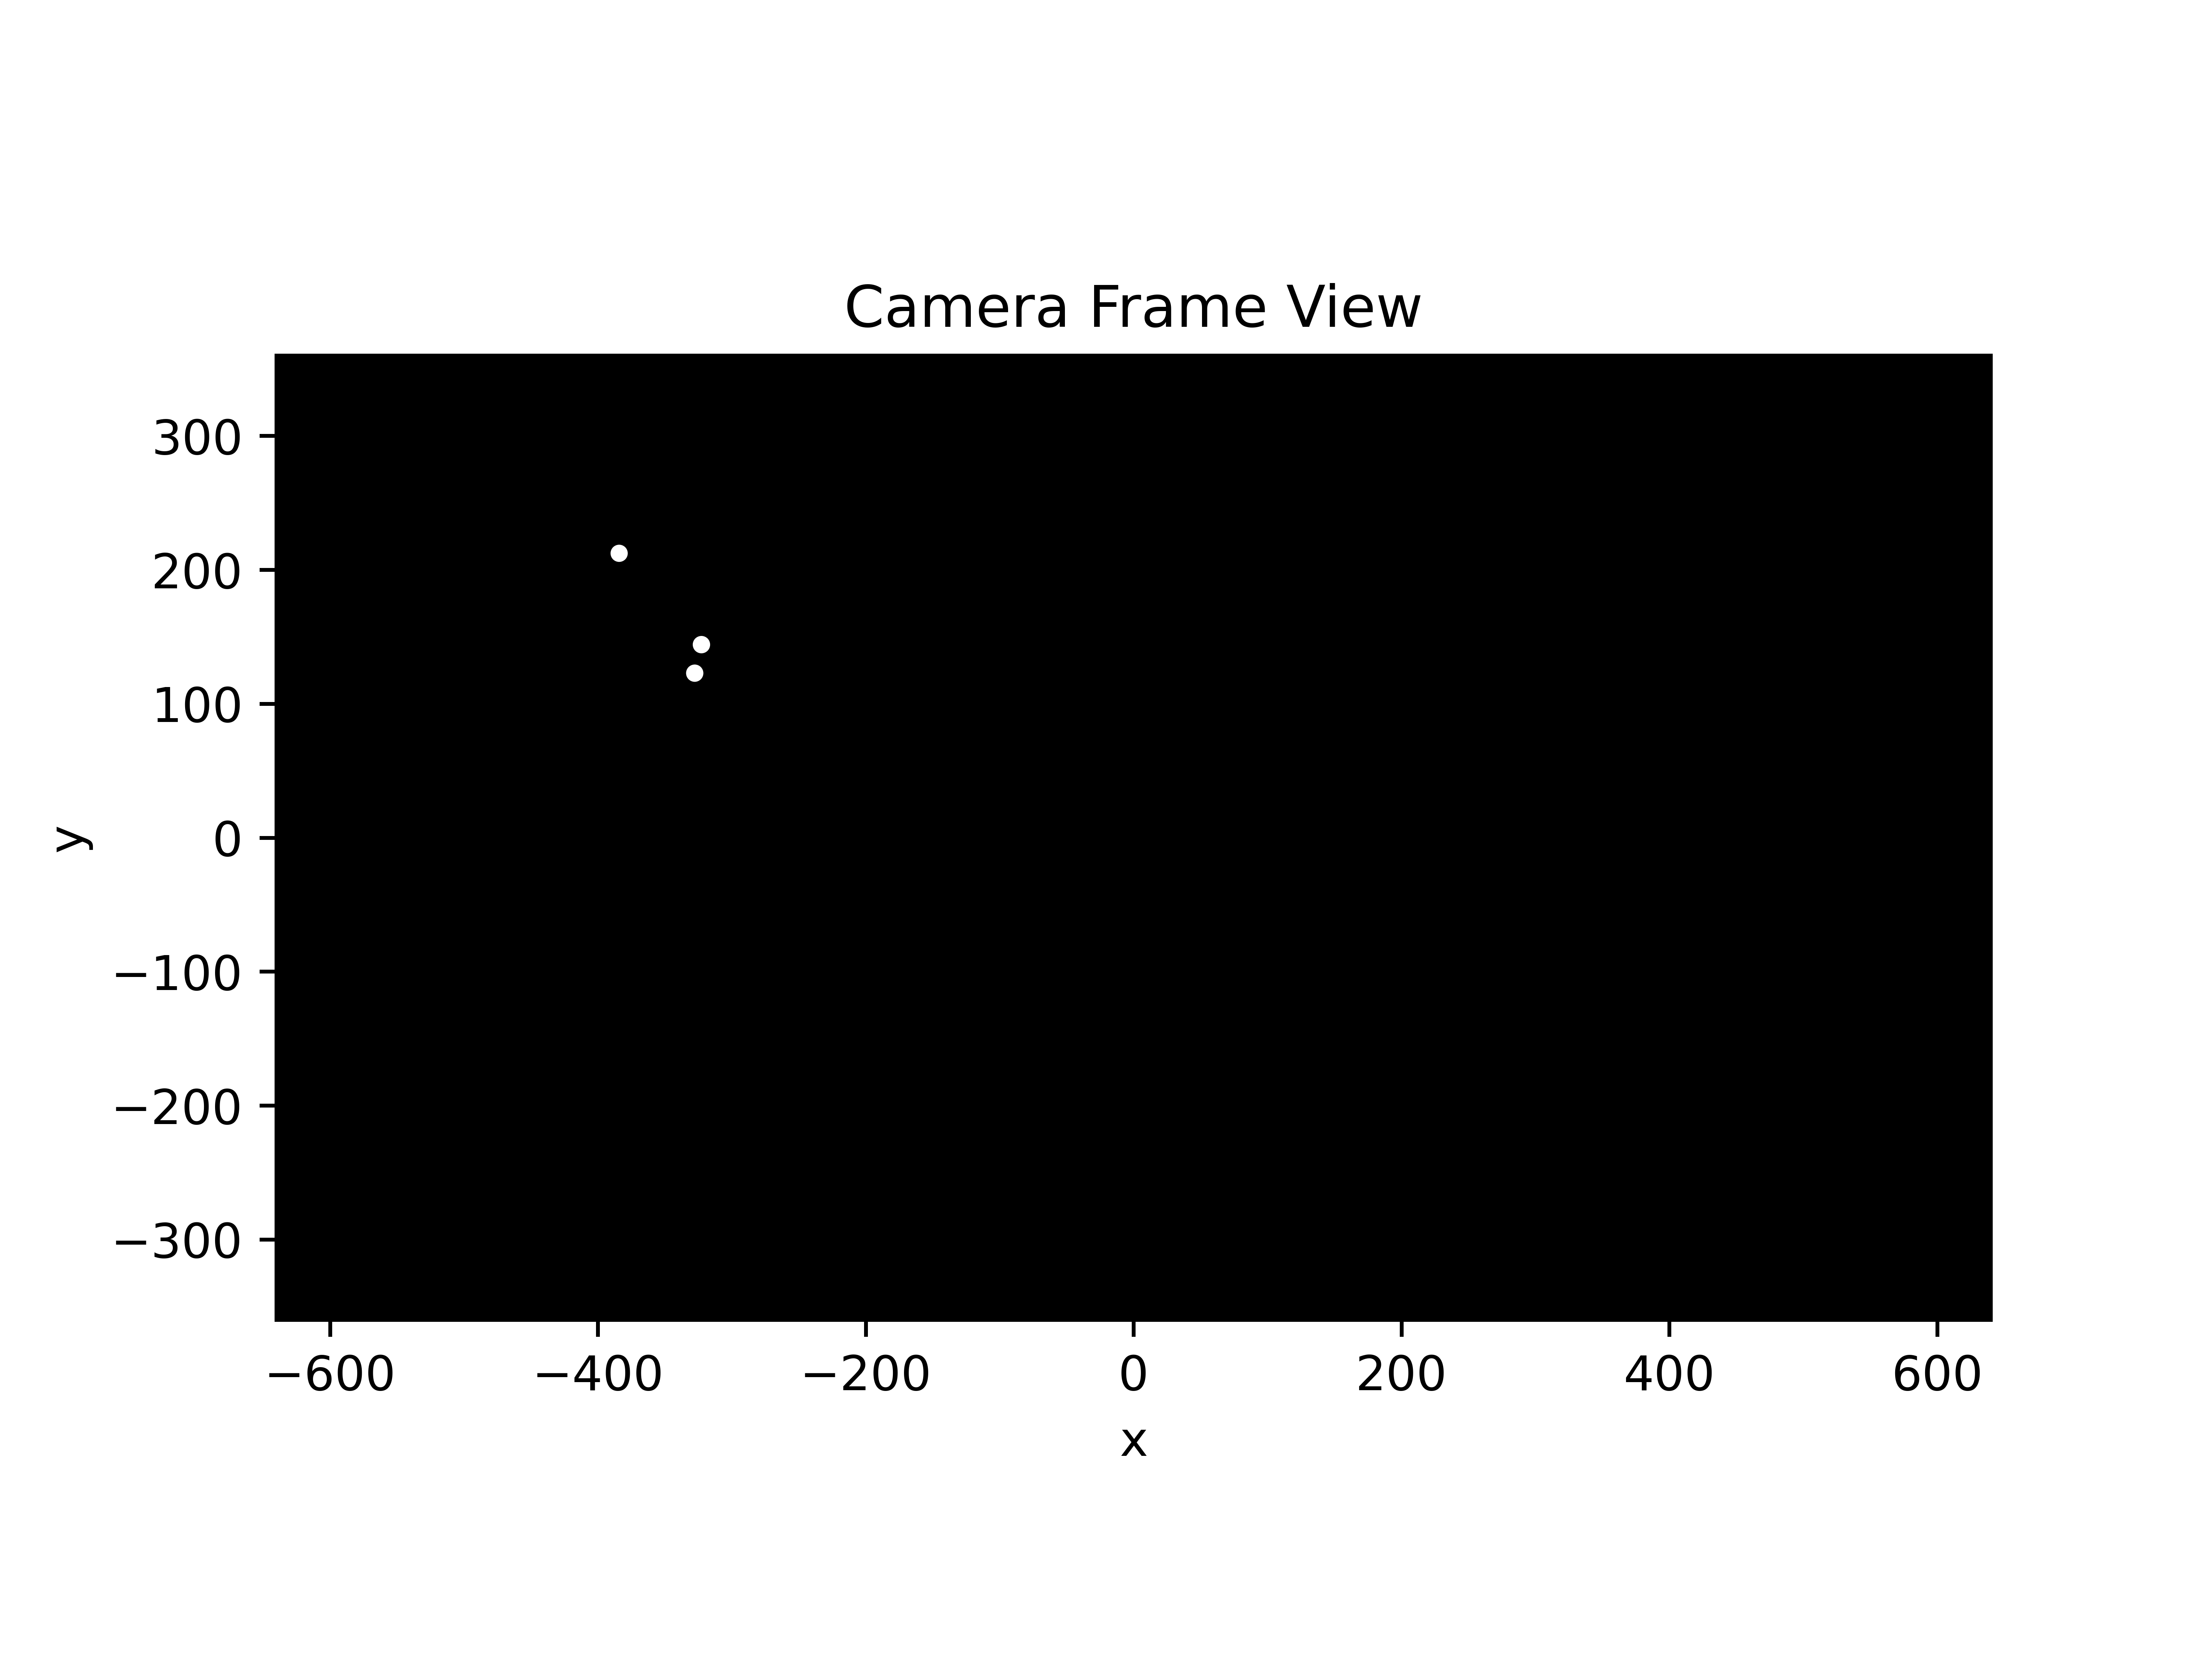
\includegraphics[width=1\textwidth]{images/acertou_2D.png}
    \caption{Resultado obtido para o caso em que o sistema detectou corretamente as estrelas presentes no FOV, Fonte: Autoria própria}
    \label{fig:acertou_2D}
\end{figure}

\begin{figure}[H]
    \centering
    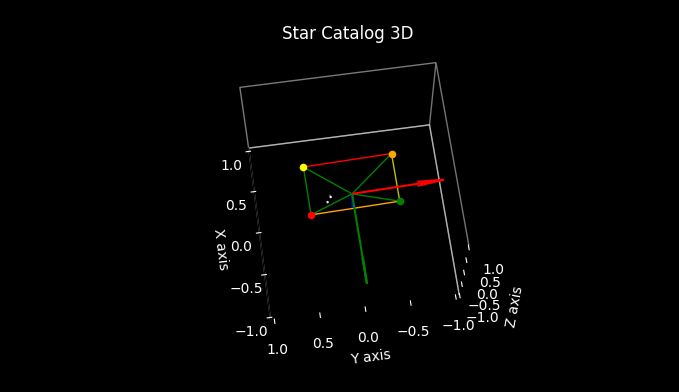
\includegraphics[width=1\textwidth]{images/acertou_3D.png}
    \caption{Resultado obtido para o caso em que o sistema detectou corretamente as estrelas presentes no FOV, Fonte: Autoria própria}
    \label{fig:acertou_3D}
\end{figure}

O resultado obtido para o caso em que o sistema detectou incorretamente as estrelas presentes no FOV,
pode ser explicado pelo fato por erros na correção das distorções da imagem,
assim como pequenos erros na localização dos centroides das estrelas.
Isto é decorrentes de erros no algorítimo de detecção de bordas aliado ao Hough Transform.

Porém, tal problema já era esperado, pois trabalhos como o de ~\cite{Cole},
já haviam demonstrado que start trackers possuem erros em algumas situações, como pode ser visto na Figura ~\ref{fig:me_salva},
porem estes erros são corrigidos em um momento posterior com a analise do proximo frame.

\begin{figure}[H]
    \centering
    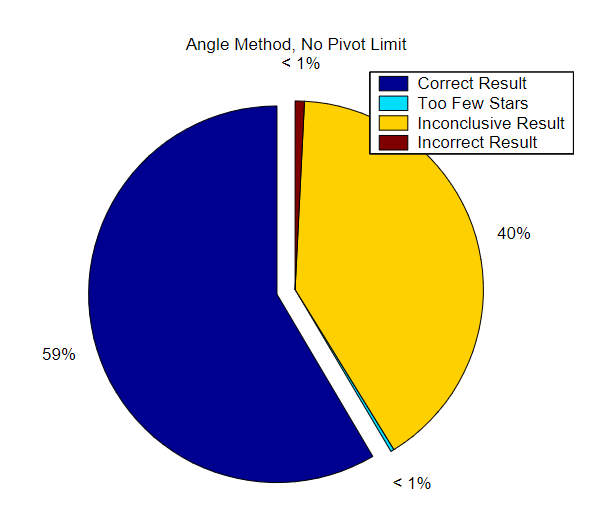
\includegraphics[width=.8\textwidth]{images/me_salva.png}
    \caption{Resultado geral de funcionamento do sistema, Fonte: ~\cite{Cole}}
    \label{fig:me_salva}
\end{figure}



\section{Códigos Fontes}

Os trabalhos desenvolvidos neste projeto estão disponíveis em 3 repositórios no GitHub, sendo eles:

\begin{itemize}
    \item \textbf{\textit{star tracker cubesat}}: Contém a implementação dos algorítimos que rodam diretamente no Cubesat, 
    juntamente dos códigos da interface utilizada para testar estes algorítimos, disponível em: ~\cite[]{Parreira_star_tracker_cubesat_2022};
    \item \textbf{\textit{star tracker simulator}}: Contém a implementação do simulador implementado em Python, 
    juntamente do executável desta simulação, disponível em: ~\cite[]{Parreira_Star_Tracker_Simulator_2022};
    \item \textbf{\textit{star tracker documentation}}: Contém a documentação do projeto, 
    incluindo o código fonte em latex, do presente documento, assim como outros dados auxiliares, 
    como os dados NASA I/239, e demais documentos disponível em: ~\cite[]{rep_documentation}.
\end{itemize}

Além disto também foi disponibilizado um vídeo demonstrando o funcionamento do sistema, disponível em: ~\cite[]{video}.